\documentclass{beamer}
\usepackage[latin1]{inputenc}
\usepackage{tikz,pgfplots}
\usetikzlibrary{arrows.meta}
\tikzset{>={Latex[width=2ex,length=2ex]}}
\pgfplotsset{compat=1.14}
\usepackage{chronology}
\tikzset{eventlabel/.append style={rotate=15}}
\tikzset{chronevent/.append style={fill=darkred}}
%\usepackage{verbatim}
\usetheme{CambridgeUS}
\title{A look At The Elephant's Tail}
\author{Gregory Stark}
\date{September 14th 2016}

%\DefineVerbatimEnvironment{GitCommit}{Verbatim}{fontfamily=tt,fontsize=\small}
%\newenvironment{GitCommit}{\begin{semiverbatim}}{\end{semiverbatim}}

\setbeamertemplate{footline}{
\begin{chronology}[2]{1995}{2017}{\textwidth}[0.9\textwidth]
  \event{\decimaldate{1}{5}{1995}}{}%Postgres95 0.1}
  \event{\decimaldate{25}{5}{1995}}{}%Postgres95 0.2}
  \event{\decimaldate{21}{7}{1995}}{}%Postgres95 0.3}
  \event{\decimaldate{5}{9}{1995}}{1.0}
  \event{\decimaldate{23}{2}{1996}}{}%Postgres95 1.01}
  \event{\decimaldate{1}{8}{1996}}{}%Postgres95 1.02}
  \event{\decimaldate{4}{11}{1996}}{}%Postgres95 1.09}
  \event{\decimaldate{29}{1}{1997}}{6.0}
  \event{\decimaldate{8}{6}{1997}}{}%6.1}
  \event{\decimaldate{2}{10}{1997}}{}%6.2}
  \event{\decimaldate{1}{3}{1998}}{6.3}
  \event{\decimaldate{30}{10}{1998}}{}%6.4}
  \event{\decimaldate{9}{6}{1999}}{6.5}
  \event{\decimaldate{8}{5}{2000}}{7.0}
  \event{\decimaldate{13}{4}{2001}}{7.1}
  \event{\decimaldate{4}{2}{2002}}{7.2}
  \event{\decimaldate{27}{11}{2002}}{7.3}
  \event{\decimaldate{17}{11}{2003}}{7.4}
  \event{\decimaldate{19}{1}{2005}}{8.0}
  \event{\decimaldate{8}{11}{2005}}{8.1}
  \event{\decimaldate{5}{12}{2006}}{8.2}
  \event{\decimaldate{4}{2}{2008}}{8.3}
  \event{\decimaldate{1}{7}{2009}}{8.4}
  \event{\decimaldate{20}{9}{2010}}{9.0}
  \event{\decimaldate{12}{9}{2011}}{9.1}
  \event{\decimaldate{10}{9}{2012}}{9.2}
  \event{\decimaldate{9}{9}{2013}}{9.3}
  \event{\decimaldate{18}{12}{2014}}{9.4}
  \event{\decimaldate{7}{1}{2016}}{9.5}
\end{chronology}
}{}

\begin{document}

\begin{frame}[plain]
  \titlepage
\end{frame}

\section{Why}
\begin{frame}{Why}
  \begin{itemize}%[<+-| alert@+>]
  \item Understanding ``who'', ``when'', and ``why'' for the decisions made
    over the past 20 years helps understand how Postgres behaves the way
    it does today including the features and limitations of the current
    code.
  \item Many of the changes fixed real problems that users faced with,
    and examining past problems helps us understand how to recognize and
    deal with problems in the future
  \item Put yourself in the shoes of an admin considering these upgrades
    and consider not just the risks of upgrading but the risks of
    \textbf{not} upgrading.
  \end{itemize}
\end{frame}


%XYZZY% \section{In the beginning}
%XYZZY% 
%XYZZY% \begin{frame}{In the beginning}
%XYZZY%   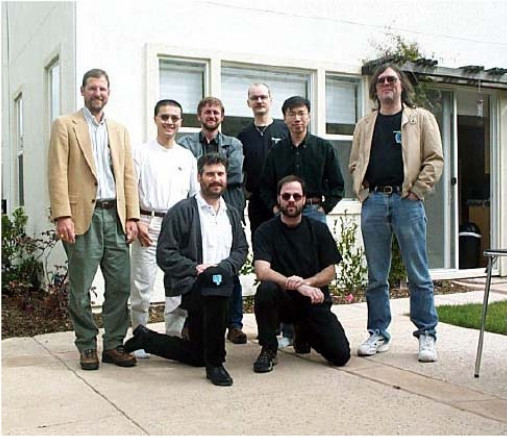
\includegraphics[width=\textwidth,height=\textheight,keepaspectratio=true]{assets/Get_to_know_PostgreSQL-6-team}
%XYZZY% \end{frame}
%XYZZY% 
%XYZZY% \begin{frame}{Postgres95 -- First Public Release}
%XYZZY%   \begin{itemize}%[<+-| alert@+>]
%XYZZY%   \item Tables limited to 1GB
%XYZZY%   \item Sorts were always on disk and always generated a new data file
%XYZZY%     for output. They always required three times as much disk space as
%XYZZY%     data being sorted
%XYZZY%   \end{itemize}
%XYZZY% \end{frame}
%XYZZY% 
%XYZZY% \begin{frame}[fragile]{Postgres 6.2 -- Use quicksort when data fits in memory}
%XYZZY%   \begin{columns}
%XYZZY%     \begin{column}{.25\textwidth}
%XYZZY%       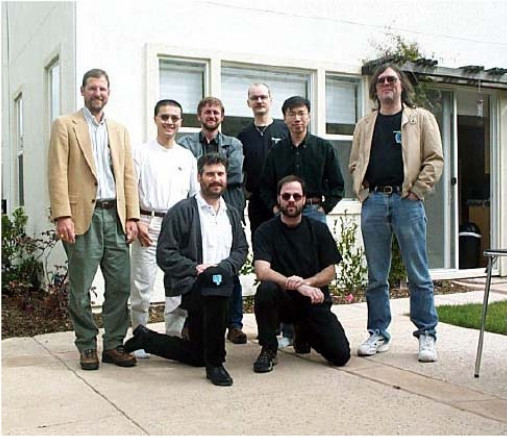
\includegraphics[width=\textwidth,height=\textheight,keepaspectratio=true]{assets/Get_to_know_PostgreSQL-6-team}
%XYZZY%     \end{column}
%XYZZY%     \begin{column}{.75\textwidth}
%XYZZY% \begin{semiverbatim}
%XYZZY% \tiny
%XYZZY%   commit 712ea2507ef7f3ea4a7149962c85de0b35245a64
%XYZZY%   Author: Vadim B. Mikheev <vadim4o@yahoo.com>
%XYZZY%   Date:   Thu Sep 18 05:37:31 1997 +0000
%XYZZY% 
%XYZZY%       1. Use qsort for first run
%XYZZY%       2. Limit number of tuples in leftist trees:
%XYZZY%           - put one tuple from current tree to disk if limit reached;
%XYZZY%           - end run creation if limit reached by nextrun.
%XYZZY%       3. Avoid mergeruns() if first run is single one!
%XYZZY% \end{semiverbatim}
%XYZZY%     \end{column}
%XYZZY%   \end{columns}
%XYZZY% \end{frame}
%XYZZY% 
%XYZZY% 
%XYZZY% %\begin{frame}{PGFPlots Bar Plot Example}
%XYZZY% %  \begin{figure}[h]
%XYZZY% %    \centering
%XYZZY% %    \begin{tikzpicture}
%XYZZY% %      \begin{axis}[
%XYZZY% %          ybar,
%XYZZY% %          enlarge x limits=0.15,
%XYZZY% %          legend style={at={(-.5,0.5)},
%XYZZY% %            anchor=north,legend columns=1},
%XYZZY% %          ylabel={\% students},
%XYZZY% %          symbolic x coords={A, B, C, D, E, F, DNF},
%XYZZY% %          xtick=data,
%XYZZY% %          bar width=2mm,
%XYZZY% %          width=0.7\textwidth
%XYZZY% %        ]
%XYZZY% %        \legend{2012, 2013};
%XYZZY% %        % Spring 2012 results
%XYZZY% %        \addplot[fill=gray]  coordinates {(A,0) (B,0) (C,3.85) (D,23.07) (E,43.31) (F,30.77) (DNF,0.00)};
%XYZZY% %        % Spring 2013 results
%XYZZY% %        \addplot[fill=blue]   coordinates {(A,0) (B,3.70) (C,22.22) (D,22.22) (E,40.74) (F,3.70) (DNF,7.41)};
%XYZZY% %      \end{axis}
%XYZZY% %    \end{tikzpicture}
%XYZZY% %    \caption{Consistent improvement over the last year}
%XYZZY% %  \end{figure}
%XYZZY% %\end{frame}
%XYZZY% 

\section{Early production use}
\begin{frame}{Postgres 7.0}
\end{frame}
\begin{frame}{Postgres 7.1}
\end{frame}
\begin{frame}{Postgres 7.2}
\end{frame}
\begin{frame}{Postgres 7.3}
\end{frame}
\begin{frame}{Postgres 7.4}
\end{frame}

%XYZZY% 
%XYZZY% \section{Middle ages}
%XYZZY% \begin{frame}{Postgres 8.0}
%XYZZY% \end{frame}
%XYZZY% \begin{frame}{Postgres 8.1}
%XYZZY% \end{frame}
%XYZZY% \begin{frame}{Postgres 8.2}
%XYZZY% \end{frame}
%XYZZY% \begin{frame}{Postgres 8.3}
%XYZZY% \end{frame}
%XYZZY% \begin{frame}{Postgres 8.4}
%XYZZY% \end{frame}
%XYZZY% 
%XYZZY% \section{Contemporary Postgres}
%XYZZY% \begin{frame}{Postgres 9.0}
%XYZZY% \end{frame}
%XYZZY% \begin{frame}{Postgres 9.1}
%XYZZY% \end{frame}
%XYZZY% \begin{frame}{Postgres 9.2}
%XYZZY% \end{frame}
%XYZZY% \begin{frame}{Postgres 9.3}
%XYZZY% \end{frame}
%XYZZY% \begin{frame}{Postgres 9.4}
%XYZZY% \end{frame}
%XYZZY% \begin{frame}{Postgres 9.5}
%XYZZY% \end{frame}
%XYZZY% \begin{frame}{Postgres 9.6}
%XYZZY% \end{frame}
%XYZZY% 
%XYZZY% \section{The future}
%XYZZY% \begin{frame}{Postgres 10}
%XYZZY% \end{frame}

\end{document}
